\pandocbounded{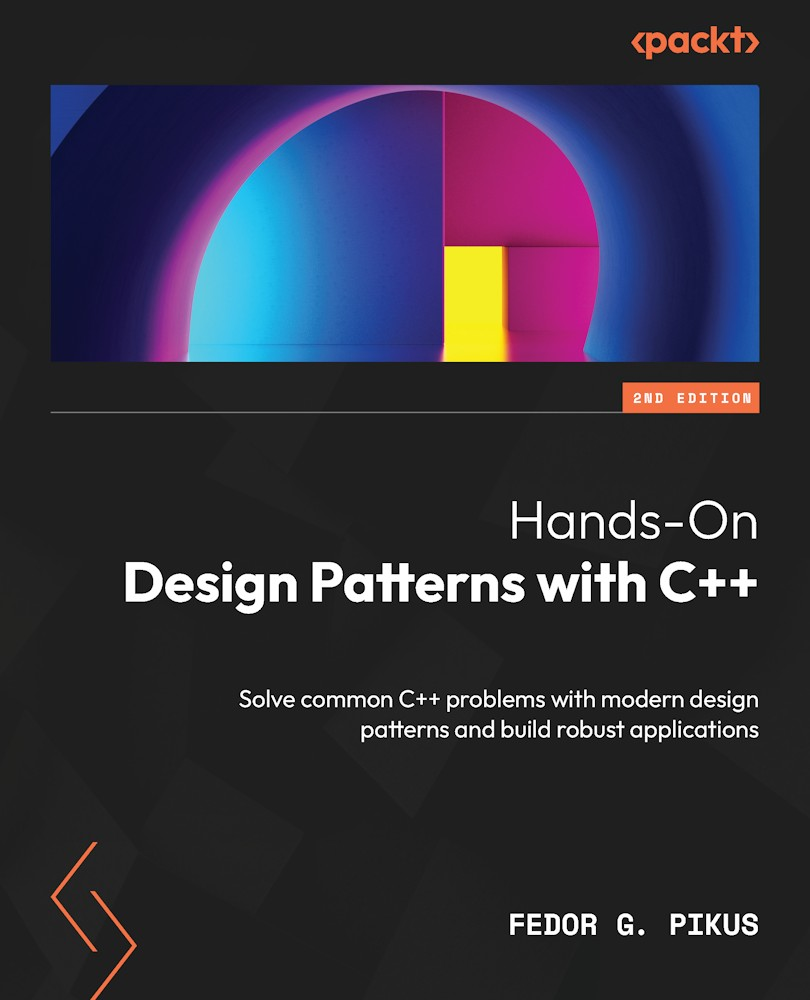
\includegraphics[keepaspectratio]{./image/Cover.png}}

\protect\phantomsection\label{B19262_FM.xhtml}{}

\section{Hands-On Design Patterns with C++}

Solve common C++ problems with modern design patterns and build robust applications

Fedor G. Pikus

\pandocbounded{
\includegraphics[keepaspectratio]{./image/Packt_Logo_SuperSite_2022_Orange.png}}

BIRMINGHAM---MUMBAI

\section{Hands-On Design Patterns with C++}

Copyright © 2023 Packt Publishing

\emph{All rights reserved}. No part of this book may be reproduced, stored in a retrieval system, or transmitted in any form or by any means, without the prior written permission of the publisher, except in the case of brief quotations embedded in critical articles or reviews.

Every effort has been made in the preparation of this book to ensure the accuracy of the information presented. However, the information contained in this book is sold without warranty, either express or implied. Neither the author(s), nor Packt Publishing or its dealers and distributors, will be held liable for any damages caused or alleged to have been caused directly or indirectly by this book.

Packt Publishing has endeavored to provide trademark information about all of the companies and products mentioned in this book by the appropriate use of capitals. However, Packt Publishing cannot guarantee the accuracy of this information.

\textbf{Associate Group Product Manager}: Kunal Sawant

\textbf{Publishing Product Manager}: Kunal Sawant

\textbf{Content Development Editor}: Rosal Colaco

\textbf{Technical Editor}: Maran Fernandes

\textbf{Copy Editor}: Safis Editing

\textbf{Project Manager}: Prajakta Naik

\textbf{Project Coordinator}: Manisha Singh

\textbf{Proofreader}: Safis Editing

\textbf{Indexer}: Manju Arasan

\textbf{Production Designer}: Prashant Ghare

\textbf{Business Development Executive}: Kriti Sharma

\textbf{Developer Relations Marketing Executives}: Rayyan Khan and Sonia Chauhan

First published: June 2019

Second edition: June 2023

Production reference: 1300623

Published by Packt Publishing Ltd.

Livery Place

35 Livery Street

Birmingham

B3 2PB, UK.

ISBN 978-1-80461-155-5

www.packtpub.com

\section{Contributors}

\section{About the author}

\textbf{Fedor G. Pikus} is a Technical Fellow and head of the Advanced Projects Team in Siemens Digital Industries Software. His responsibilities include planning the long-term technical direction of Calibre products, directing and training the engineers who work on these products, design, and architecture of the software, and researching new design and software technologies.

His earlier positions included a Chief Scientist at Mentor Graphics (acquired by Siemens Software), a Senior Software Engineer at Google, and a Chief Software Architect for Calibre Design Solutions at Mentor Graphics. He joined Mentor Graphics in 1998 when he made a switch from academic research in computational physics to the software industry.

Fedor is a recognized expert in high-performance computing and C++. He is the author of two books on C++ and software design, has presented his works at CPPNow, CPPCon, SD West, DesignCon, and in software development journals, and is also an O'Reilly author. Fedor has over 30 patents and over 100 papers and conference presentations on physics, EDA, software design, and C++ language.

This book would not be possible without the support of my wife, Galina, who made me go on in moments of self-doubt. Thank you to my sons, Aaron and Benjamin, for their enthusiasm. I especially appreciate my cats, Pooh and Tux, for letting me use their warming pad as my laptop.

\section{About the reviewer}

\textbf{Andrey Gavrilin} is a senior software engineer working for an international company that provides treasury management cloud solutions. He has an MSc degree in engineering (industrial automation) and has worked in different areas such as accounting and staffing, road data bank, web and Linux distribution development, and fintech. His interests include mathematics, electronics, embedded systems, full-stack web development, retro gaming, and retro programming.

\protect\phantomsection\label{B19262_TOC_ePub.xhtml}{}

\protect\phantomsection\label{B19262_Preface.xhtml}{}

\section{Preface}

When considering this book, some of you will ask: \emph{Another book on design patterns in C++? Why that, and why now? Hasn't everything there is to know about design patterns been} \emph{written already?}

There are several reasons why yet another book on \emph{design} \emph{patterns} has been written, but first of all, this is very much a C++ book---this is not a book on \emph{design patterns} in C++ but a book on design patterns \emph{in C++}, and the emphasis sets it apart. C++ has all the capabilities of a traditional object-oriented language, so all the classic object-oriented design patterns, such as Factory and Strategy, can be implemented in C++. A few of those are covered in this book. But the full power of C++ is realized when you utilize its generic programming capabilities. Remember that design patterns are frequently occurring design challenges and the commonly accepted solution---both sides are equally important in a pattern. It stands to reason that when new tools become available, new solutions become possible. Over time, the community settles on some of these solutions as the most advantageous overall, and a new variation of an old design pattern is born---the same challenge but a different preferred solution. But expanding capabilities also opens up new frontiers---with new tools at our disposal, new design challenges arise.

Others may expect to find a new coming of the classic book ``\emph{Design Patterns: Elements of Reusable Object-Oriented Software}''. This `isn't that book, and I do not believe that the time is right for such a book. The ``\emph{Gang of Four}'' book was novel, even revolutionary, and it introduced the language of design patterns into the broad programming community. This has been done once and for all. It also established the neat taxonomy of design patterns, and that part has not aged nearly as well: as our pattern vocabulary expanded, we found patterns that do not fit easily into a particular category. We also extended the notion of design patterns beyond object-oriented programming and found that some of these patterns strongly resemble their object-oriented cousins while others are entirely new and different. Furthermore, in C++ and other languages with significantly different capabilities, a pattern that addresses the same need may look totally different. The bottom line is the original classification of patterns, while still useful, by now has more exceptions than typical examples, and the pattern landscape became too divergent for a new taxonomy that would not seem far too artificial. Maybe in time, as we develop the art further, new trends will emerge from the bird's eye view of the expanded pattern landscape, but it has not happened yet.

This book has less ambitious but very practical goals. In this book, we focus on design patterns where C++ has something essential to add to at least one of the two sides of the pattern. On the one hand, we have patterns such as Visitor, where the generic programming capabilities of C++ allow for a better solution. That better solution was made possible by new features that were added with the evolution of the language from C++11 to C++17. On the other hand, generic programming is still programming (only the execution of the program happens at compile time); programming requires design, and design has common challenges that are not all that dissimilar to the challenges of traditional programming. Thus, many of the traditional patterns have their twins, or at least close siblings, in generic programming, and we largely focus on those patterns in this book. A prime example is the Strategy pattern, better known in the generic programming community by its alternative name, the Policy pattern. Also, as new features are added to the language, it can offer solutions to new problems or new solutions to old problems, and both of these eventually develop into design patterns. This is the case with the C++ coroutines, which make an appearance in the last chapter.

Finally, a language as complex as C++ is bound to have a few idiosyncrasies of its own that often lead to C++-specific challenges that have common, or \emph{standard}, solutions. While not quite deserving of being called \emph{patterns}, these C++-specific idioms are also covered in this book.

A few words about the changes for the second edition: first of all, there is a new chapter on patterns for concurrency. All examples are updated to use C++17 or C++20 wherever it makes sense, but never gratuitously. Many patterns, idioms, and examples demonstrating their use were updated with recent developments and advances -- the result of the work of the C++ programming community in the last few years.

All that said, there are three main reasons why this book has been written:

\begin{itemize}
\tightlist
\item
  To cover C++-specific solutions for otherwise general, \emph{classic} design patterns
\item
  To show C++-specific pattern variants that occur when old design challenges arise in the new domain of generic programming
\item
  To keep our patterns up to date with the language's evolution
\end{itemize}

\section{Who this book is for}

This book is intended for C++ programmers who want to learn from \emph{the wisdom of the community}---from commonly-recognized good solutions to frequently occurring design problems. Another way to put it is that this book is a way for a programmer to learn from someone else's mistakes.

This is not a \emph{learn} \emph{C++} book; the target audience is mostly programmers who are reasonably familiar with the tools and the syntax of the language, and who are more interested in learning how and why these tools should be used. However, this book will also be useful for programmers wanting to learn more about C++, but wishing that their study could be guided by concrete and practical examples (for such programmers, we recommend having a C++ reference book close to hand as well). Finally, programmers who want to learn not just what's new in C++17 or C++20, but what all these new features can be used for, will hopefully find this book illuminating as well.

\section{What this book covers}

\emph{Chapter 1, An Introduction to Inheritance and Polymorphism}, provides a brief overview of the object-oriented features of C++. This chapter is not intended as a reference for object-oriented programming in C++, but, rather, highlights the aspects of it that are important for the subsequent chapters.

\emph{Chapter 2, Class and Function Templates}, provides an overview of the generic programming facilities of C++---class templates, function templates, and lambda expressions. This chapter covers template instantiations and specializations, along with template function argument deduction and overload resolution, and prepares you for more complex uses of templates in later chapters.

\emph{Chapter 3, Memory and Ownership}, describes modern idiomatic ways of expressing different kinds of memory ownership in C++. This is a collection of conventions or idioms---the compiler does not enforce these rules, but programmers will find it easier to understand each other if they use the shared idiomatic vocabulary.

\emph{Chapter 4, Swap - From Simple to Subtle}, explores one of the most basic C++ operations, the swap, or exchange, of two values. This operation has surprisingly complex interactions with other C++ features that are discussed in the chapter.

\emph{Chapter 5, A Comprehensive Look at RAII}, explores in detail one of the fundamental concepts of C++, that of resource management, and introduces what may be the most popular C++ idiom, RAII, which is the standard C++ approach to managing resources.

\emph{Chapter 6, Understanding Type Erasure}, provides insight into a C++ technique that has been available in C++ for a long time but has grown in popularity and importance since the introduction of C++11. Type erasure allows the programmer to write abstract programs that do not explicitly mention certain types.

\emph{Chapter 7, SFINAE, Concepts, and Overload Resolution Management}, discusses SFINAE---a C++ idiom that is, on the one hand, essential to the use of templates in C++ and \emph{just happens} transparently, while on the other hand, requires a very thorough and subtle understanding of C++ templates when used purposefully.

\emph{Chapter 8, The Curiously Recurring Template Pattern}, describes a \emph{mind-wrapping} template-based pattern that combines the benefits of object-oriented programming with the flexibility of templates. The chapter explains the pattern and teaches you how to use it properly to solve practical problems. Lastly, this chapter prepares you for recognizing this pattern in later chapters.

\emph{Chapter 9, Named Arguments, Method Chaining, and the Builder Pattern}, covers an unusual technique for calling functions in C++, using named arguments instead of positional ones. This is another one of those idioms we use implicitly in every C++ program, but its explicit purposeful use takes some thought.

\emph{Chapter 10, Local Buffer Optimization}, is the only purely performance-oriented chapter in this book. Performance and efficiency are critical considerations that influence every design decision that affects the language itself---there is not a feature in the language that was not reviewed from the point of view of efficiency before being accepted into the standard. It is only fair that a chapter is dedicated to a common idiom used to improve the performance of C++ programs.

\emph{Chapter 11, ScopeGuard}, introduces an old C++ pattern that has changed almost beyond recognition with the recent versions of C++. The chapter teaches you about a pattern for easily writing exception-safe, or, more generally, error-safe code in C++.

\emph{Chapter 12, Friend Factory}, describes another old pattern that finds new uses in modern C++. This pattern is used to generate functions \emph{associated} with templates, such as arithmetic operators for every type generated by a template.

\emph{Chapter 13, Virtual Constructors and Factories}, covers another classic object-oriented programming pattern as applied to C++, the Factory pattern. In the process, the chapter also shows you how to get the appearance of polymorphic behavior from C++ constructors, even though constructors cannot be virtual.

\emph{Chapter 14, The Template Method Pattern and the Non-Virtual Idiom}, describes an interesting crossover between a classic object-oriented pattern, the template, and a very C++-centric idiom. Together, they form a pattern that describes the optimal use of virtual functions in C++.

\emph{Chapter 15, Policy-Based Design}, covers one of the jewels of C++ design patterns, the Policy pattern (more commonly known as the Strategy pattern), applied at compile time, that is, as a generic programming pattern instead of an object-oriented pattern.

\emph{Chapter 16, Adapters and Decorators}, discusses the two very broad and closely related patterns as they apply to C++. The chapter considers the use of these patterns in object-oriented designs, as well as in generic programs.

\emph{Chapter 17, The Visitor Pattern and Multiple Dispatch}, rounds off our gallery of classic object-oriented programming patterns with the perennially popular Visitor pattern. The chapter explains the pattern itself, then focuses on the ways that modern C++ makes the implementation of Visitor simpler, more robust, and less error-prone.

\emph{Chapter 18, Patterns for Concurrency}, is a new addition to the book. While C++ has been used to write concurrent programs long before C++11 gave us the ``official'' tools for it, the wide range of problem-specific solutions makes identifying common patterns difficult. This chapter introduces the patterns that became the basic building blocks for designing concurrent software in C++.

\section{To get the most out of this book}

To run examples from this book, you will need a computer running Windows, Linux, or macOS (C++ programs can be built on something as small as a Raspberry Pi). You will also need a modern C++ compiler, such as GCC, Clang, Visual Studio, or another compiler that supports the C++ language up to C++20 (most examples need only C++14, some rely on C++17 features, and a few require up-to-date C++20 support). You will need a basic knowledge of GitHub and Git in order to clone a project with examples.

\section{Download the example code files}

You can download the example code files for this book from GitHub at https://github.com/PacktPublishing/Hands-On-Design-Patterns-with-CPP-Second-Edition/. If there's an update to the code, it will be updated in the GitHub repository.

We also have other code bundles from our rich catalog of books and videos available at https://github.com/PacktPublishing/. Check them out!

\section{Conventions used}

There are a number of text conventions used throughout this book.

\texttt{Code\ in\ text}: Indicates code words in text, database table names, folder names, filenames, file extensions, pathnames, dummy URLs, user input, and Twitter handles. Here is an example: ``The implementation of the \texttt{insert()} function must insert the record into both the storage and the index, there is no way around it.''

A block of code is set as follows:

\begin{verbatim}

class Database {
  class Storage { ... };    // Disk storage Storage S;
  class Index { ... };    // Memory index Index I;
  public:
  void insert(const Record& r);
  ...
};
\end{verbatim}

Any command-line input or output is written as follows:

\begin{verbatim}

Benchmark                              Time
-------------------------------------------
BM_delete_explicit                  4.54 ns
BM_delete_type_erased               13.4 ns
BM_delete_type_erased_fast          12.7 ns
BM_delete_template                  4.56 ns
\end{verbatim}

Tips or important notes

Appear like this.

\section{Get in touch}

Feedback from our readers is always welcome.

\textbf{General feedback}: If you have questions about any aspect of this book, email us at customercare@packtpub.com and mention the book title in the subject of your message.

\textbf{Errata}: Although we have taken every care to ensure the accuracy of our content, mistakes do happen. If you have found a mistake in this book, we would be grateful if you would report this to us. Please visit www.packtpub.com/support/errata and fill in the form.

\textbf{Piracy}: If you come across any illegal copies of our works in any form on the internet, we would be grateful if you would provide us with the location address or website name. Please contact us at copyright@packt.com with a link to the material.

\textbf{If you are interested in becoming an author}: If there is a topic that you have expertise in and you are interested in either writing or contributing to a book, please visit authors.packtpub.com.

\section{Share Your Thoughts}

Once you've read \emph{Hands-On Design Patterns with C++ (Second Edition)}, we'd love to hear your thoughts! Please click here to go straight to the Amazon review page for this book and share your feedback.

Your review is important to us and the tech community and will help us make sure we're delivering excellent quality content.

\section{Download a free PDF copy of this book}

Thanks for purchasing this book!

Do you like to read on the go but are unable to carry your print books everywhere?

Is your eBook purchase not compatible with the device of your choice?

Don't worry, now with every Packt book you get a DRM-free PDF version of that book at no cost.

Read anywhere, any place, on any device. Search, copy, and paste code from your favorite technical books directly into your application.

The perks don't stop there, you can get exclusive access to discounts, newsletters, and great free content in your inbox daily

Follow these simple steps to get the benefits:

\begin{enumerate}
\tightlist
\item
  Scan the QR code or visit the link below
\end{enumerate}

\pandocbounded{
\includegraphics[keepaspectratio]{./image/B19262_QR_Free_PDF.jpg}}

https://packt.link/free-ebook/9781804611555

\begin{enumerate}
\tightlist
\item
  Submit your proof of purchase
\item
  That's it! We'll send your free PDF and other benefits to your email directly
\end{enumerate}

\protect\phantomsection\label{B19262_Part_01.xhtml}{}